\chapter{ピューリッツァー賞作家が語る創作のプロセス --- Richard Powers}

この講義は二度始まる。まず圧縮された格言が置かれる。登場人物を壁際まで追いつめれば、そこにドラマが現れるのだ、と。ついで会話は、より辛抱強く、地ならしするように再開される。主題となる地形、すなわちドラマ、葛藤、声、対話に名が与えられ、その主張が日常の社会生活から外側へ向かって組み直されていく。この二重の始まりは重要である。私たちはまず答えを与えられ、そのあとで仕組みを示される。したがって、このノートの課題は、その律動を保つことにある。まず圧力、それから人物、ついで葛藤の拡大する尺度、そしてそのあとにはじめて、言葉、統語法、緊張、推敲といった微細な craft へ降りていくのである。

\section{人物、圧力、そしてドラマの三つの水準}

Powers は、劇作家がそうあるべき場所から始める。プロットの機械仕掛けからではなく、緊張のもとに置かれたひとりの人間からである。人物とは複雑なものだ、と彼は言う。そしてその複雑さは、状況が選択を強いるときにしか本当には見えてこない。これが cold-open の thesis であり、最も圧縮された形では
\begin{equation}
\text{人物} \Rightarrow \text{ドラマ}.
\end{equation}
と書ける。ここは注意して聞くべきである。この主張は、ドラマが外から人物に貼りつけられるという意味ではない。主張されているのは、圧力が十分に高まったときにしか、人物は可読的にならないということだ。何ひとつ賭けられていなければ、私たちは traits や surfaces や manner を得るかもしれないが、necessity は得られない。

講義は次に、好んで用いるあの escalation の一つを行う。私たちはまず、人が自己と争うこと、人が他者と争うことから始める。それで尽きるのか。そうではない。もう一つ、第三の尺度がある。Powers はその全階梯を次のように名づける。
\begin{equation}
\text{person vs self},\qquad \text{person vs person},\qquad \text{person vs world}.
\end{equation}
第一は内面的衝突である。第二は社会的・政治的衝突である。第三は、人間の企てと、その企てが生きねばならないより大きな世界との衝突である。

cold open のあと、interview は別の調子で再開され、講義最初の大きな動機づけを与える。人物とは、異様な literary invention ではない。私たちはすでにそれを、日々たえず行っているのだ。人間は、他者の隠れた動機、古い遺恨、語られない郷愁、別の未来を推測することによって、社会の中で生き延びている。私たちは、それぞれの生活の中ですでに皆、小説家なのだと Powers は言う。fiction は、日常生活がすでに鍛えている能力を洗練するのである。

だからこそ、講義は次に抽象ではなく、生きた fictional examples へ向かう。Powers は \emph{Playground} の protagonists である Todd Keen と Rafael について語る。彼らは、自分自身の過去に残された未完の素材同士を、劇化された形で衝突させることのできる figures だったのである。要点は、単なる autobiography ではない。要点は、人物はいったん十分に活動し始めると、自然に conflict へ向かうということだ。友情、 rivalries、不信、階級差、相互依存。これらは人物の周囲に置かれた decoration ではない。ドラマが育ち始める局所的な形なのである。

\subsection{Question \& Answer}

\paragraph{Question.} ドラマは実際にはどこから来るのか。

\paragraph{Answer.} 避けがたくなった衝突から来る。人物が壁際まで押しやられ、二つの価値が両立できなくなり、二人の人間が異なるものを必要とし、あるいは人間の企てがより大きな世界にぶつかるのだ。``壁際まで追いつめよ'' とは、単なる intensity についての助言ではない。講義における最初の本当の method なのである。

\section{人物という onion: traits、mannerisms、core inner values}

Powers は、人物が日常生活の中にすでに潜んでいると私たちに納得させたあとで、直観から procedure へと向きを変える。ここで講義は、明示的に pedagogical になり、Stanislavski に寄りかかる。俳優も、小説家も同じく、自分自身と同一ではないひとりの人間の内側に住まなければならない。それは模倣だけによってではなく、より inward で fundamental な何かを見つけ、そこへ入っていくことによって行われる。

その teaching image が onion である。外側には traits がある。その内側に mannerisms があり、さらにその奥に core inner values がある。圧縮すれば、
\begin{equation}
\text{core inner values} \to \text{mannerisms} \to \text{traits}.
\end{equation}
となる。

\begin{figure}[h]
\centering
\begin{tikzpicture}[scale=0.95]
\draw[thick] (0,0) circle (2.7);
\draw[thick] (0,0) circle (1.8);
\draw[thick] (0,0) circle (0.95);
\node at (0,2.25) {\small 特性};
\node at (0,1.35) {\small 癖や身ぶり};
\node at (0,0) {\small 中核となる内的価値};
\end{tikzpicture}
\caption{Powers の ``onion'' model of character を、transcript に基づいて再構成した schematic。}
\end{figure}

traits は外殻である。読者が最初に人物をつかむための、目に見える、あるいは performative な details だ。その殻の下に mannerisms がある。挑発、なだめ、回避、誇示、制御といった反復的な habits である。さらに深く、core inner values がある。honesty、fidelity、perseverance、freedom、equality、attentiveness、complicity。これらの values は交換可能な ornaments ではない。人物が世界の中で守ろうとしている inward な commitments なのである。

Powers は、この onion をあまり mechanical にしすぎないよう careful である。矢印は one-to-one ではない。複数の values が同じ mannerism を支えているかもしれないし、複数の mannerisms が同じ visible trait を支えているかもしれない。だからこそ characterization は inventory によって solve されない。coherence によって solve されるのである。外側の behavior は、同時に隠し、同時に明かさなければならない。

講義の Nemo の example が useful なのは、まさにこの structure を teachable にするからである。父親の overprotectiveness は、単なる trait ではない。それは、より深い commitments から出てくる visible pattern である。fear、love、protectiveness、そして再び loss を risk することの refusal。そう見えてきた瞬間、surface は単なる描写ではなく、dynamic なものになる。

\paragraph{Worked derivation.} 描写をドラマへ変えるための Powers の procedure は、短い chain として書ける。
\begin{enumerate}
\item visible な trait から始める。
\item その trait を生み出している mannerism または recurring behavior は何かを問う。
\item その mannerism を支えうる core inner value は何かを問う。
\item その人物がまた手放したがらない第二の value を加える。
\item その二つの values が両立して保たれえない situation を構築する。
\item 強制された喪失が interior drama を生む。
\end{enumerate}

だからこそ、この講義の signature example はこれほど強いのである。
\begin{equation}
\text{honesty} + \text{fidelity} + \text{forced choice} \Rightarrow \text{interior drama}.
\end{equation}
友人が何か wrong なことをした。真実を tell して友を betray するべきか。それとも loyal でいることで truth を betray するべきか。story は labels から始まるのではない。その labels がもはや coexist できなくなるときに始まるのである。

\subsection{Question \& Answer}

\paragraph{Question.} 人を mere な description ではなく、dramatic な character へ変えるにはどうすればよいか。

\paragraph{Answer.} 外へ向かう前に下へ向かうのである。traits の下に mannerisms を、mannerisms の下に values を infer する。そしてそれらの values を衝突させる。description が character になるのは、何か inward なものが選ばれねばならず、何か inward なものが失われねばならないときである。

\section{人間世界の外へ: ecological で metaphysical な drama}

この point で講義は、ふたたび scale を widen する。この move は Powers らしい。person against self、person against person で十分か。そうではない。人間は、他の人間たちと collide するだけではない。自分たちより大きな世界が set する terms ともまた collide するのである。

彼はこの widening を、次のように名づける。
\begin{equation}
\text{psychological} \to \text{sociological/political} \to \text{environmental/metaphysical}.
\end{equation}
最初の二つの kinds の drama は、多くの modern fiction において dominant であった。第三のものは、Powers によれば、しばしば thinned out されるか neglect されてきた。literary fiction は inner life と social life においてきわめて adept になった一方で、人間を、他の everything から autonomous な存在であるかのように扱うことがあまりにも多かったのである。

だからこそ講義は、literary history に real な時間を割く。昔ながらの ``man against nature'' の story は quaint に見え始めた。とはいえ myth、epic、frontier fiction、\emph{Moby-Dick}、science fiction、fantasy がその third form をほんとうに lost したことはなかった。Powers にとって dip とは、第三の drama が everywhere で disappear したことではない。何が respectable literary seriousness と count されるかが narrowed されたことなのだ。長いあいだ、serious fiction は、人間が nonhuman world との struggle にすでに勝ったかのように振る舞うことができた。ecological crisis は、その illusion を終わらせた。third drama は、world が equation の active term として return してきたために、いま戻ってきたのである。

私たちは conflict の三つの scales と、その widening field を、一本の visual line にまとめて書くことができる。
\begin{equation}
\text{person vs self} \Rightarrow \text{person vs person} \Rightarrow \text{person vs world}.
\end{equation}
ここでの arrows は、later な scale が earlier な scale を replace することを意味しない。later な scale が earlier な scale を contain し、enlarge することを意味している。

このあたりで Powers は trees、childhood animism、そして older literatures に話を向ける。この move を ``environmental themes'' に flatten してしまうのは、簡単だが間違いである。それでは弱すぎる。彼の stronger な claim は、nonhuman world への attention は、interior drama へ至る another route でもある、ということだ。子どもは、adults が wood しか見ないところに aliveness を見る。oral literatures は、人間が、自分ではないものとの conversation を抜きにしては理解できないことを知っていた。だからこそ講義には、印象的な sentence が現れる。nonhuman world を look することは、interior drama を understand することでもあるのだ、と。

Powers の science と animism の fusion は、ここから directly に follow する。私たちは world を、science が know するように know しなければならず、同時に animist な child が know するようにも know しなければならない。これらは敵対する programs ではない。どちらか一方 alone では hold しきれないほど richer な reality へアクセスする二つの ways なのである。

\subsection{Question \& Answer}

\paragraph{Question.} full scale の drama を capture するために、なぜ stories は human の外側へ move しなければならないのか。

\paragraph{Answer.} human life は self-sealed ではないからである。私たちの values や projects は、自分たちより大きな living world の内部で形を取る。その world はそれらに抵抗し、無視し、あるいは変形しうる。fiction がその dimension を omit してしまえば、それは purer になるのではない。narrower になるのである。

\section{なぜ fiction は私たちを move しうるのか: story、affect、そして value の change}

story の scale を widen したあとで、Powers は force の question へ turn する。そもそもなぜ fiction は matter しうるのか。lecture における immediate な motivation は concrete である。David は \emph{The Overstory} の passages を aloud に read し、この novel が information を beyond した何かを doing していると feel する。Powers は、その difference に great clarity で name を与える。
\begin{equation}
\text{apprehension of fact} \neq \text{shift in values}.
\end{equation}
私たちは、何かを intellectually に learn しながら、なお caring の structure においては unchanged のままでいることができる。facts は grasp されても commitments にはならない。

novel は、別の route によって work する。
\begin{equation}
\text{story} \Rightarrow \text{affect} \Rightarrow \text{identification} \Rightarrow \text{movement of the reader}.
\end{equation}
だからこそ emotion についての彼の etymological aside は matter する。emotion は、私たちが possess する mere な feeling ではない。それは、私たちを通って流れ、私たちを onward へ move するものなのだ。story は merely instruct しない。reader を another perspective の inside へ re-situate するのである。

講義はこれを、familiar な psychology experiment を通して concrete にする。details が matter する。なぜなら Powers は mystical claim をしているのではない。mechanism を describe しているのだから。

\paragraph{Worked example.} helping-behavior experiment は、次のように unfold する。
\begin{enumerate}
\item different groups の subjects が、comprehension exercise という guise のもとで、different な texts を read するよう求められる。
\item ある group は neutral material を read し、別の group は non-affective な data を read し、さらに別の group は feeling と identification を produce しうる fictional passage を read する。
\item comprehension questions に answer したあと、subjects は room を leave する。
\item hallway で、confederate が pencils を drop するか、carry していた materials を spill する。
\item moving な story を just read した group は、立ち止まって help する likelihood がより高い。
\end{enumerate}
inference は、fiction が permanently に私たちを save するということではない。もっと modest で、もっと interesting である。identification は、たとえ一瞬であれ、reader を greater sympathy と responsiveness のほうへ baseline-shift させるのである。

これが、この講義が argument と narrative との old rivalry に与える strongest な answer である。bare な argument は assent を secure するかもしれない。story は、reader が what to do を準備するその仕方を change しうる。だからこそ Powers は later に、この point を自分自身の hard maxim に compress する。best arguments が必ずしも mind を change するわけではない。good story はそうしうるのだ。

\subsection{Question \& Answer}

\paragraph{Question.} argument にはできないのに、なぜ story は reader を move しうるのか。

\paragraph{Answer.} entry の route を変えるからである。argument は belief に directly に address する。story は affect を recruit し、affect は identification を recruit する。reader が ``Who would I be if I were that person?'' と ask した瞬間、その resulting な change はもはや merely conceptual ではない。active になるのである。

\section{下から立ち上がる voice: register、diction、syntax、そして predication}

ここに来てようやく、講義は nuts and bolts へ descend する。この order は essential である。Powers は、craft trivia から begin して stakes が後から arrive するのを hope したりはしない。まず fiction が何を do するのかを tell し、そのあとではじめて、その machinery がどう work するのかを問うのである。

彼はこの descent を、lecture の strongest images の一つによって導入する。novel は、many dogs が harness で引く sled なのだ。language が一匹の dog、character が another、drama が another、form と structure がまた別の dogs である。problem は、一匹を choose して他を despise することではない。それらすべてを same direction に pull させることなのである。

したがって causal spine は、two-step である。
\begin{equation}
\text{voice} \Rightarrow \text{character},\qquad
\text{character} \Rightarrow \text{drama}.
\end{equation}
もし lecture に基づいて、より fully な transcript-based reconstruction を allow するなら、downward chain は
\begin{equation}
\text{diction/register/syntax} \Rightarrow \text{voice} \Rightarrow \text{character} \Rightarrow \text{drama} \Rightarrow \text{form}.
\end{equation}
となる。

\begin{figure}[h]
\centering
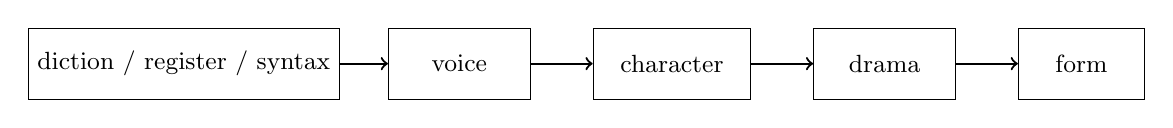
\begin{tikzpicture}[x=1cm,y=1cm]
\node[draw, minimum width=2.7cm, minimum height=0.9cm] (a) at (0,0) {\small diction / register / syntax};
\node[draw, minimum width=1.8cm, minimum height=0.9cm] (b) at (3.5,0) {\small voice};
\node[draw, minimum width=2cm, minimum height=0.9cm] (c) at (6.2,0) {\small character};
\node[draw, minimum width=1.8cm, minimum height=0.9cm] (d) at (8.9,0) {\small drama};
\node[draw, minimum width=1.6cm, minimum height=0.9cm] (e) at (11.4,0) {\small form};
\draw[->, thick] (a) -- (b);
\draw[->, thick] (b) -- (c);
\draw[->, thick] (c) -- (d);
\draw[->, thick] (d) -- (e);
\end{tikzpicture}
\caption{講義の downward craft chain を、transcript に基づいて schematic に再構成したもの。}
\end{figure}

ここで notice すべきは、その sequence である。form は、上から imposed される top-level shell ではない。lower levels における decisions から emerge するのだ。これが、この講義のもっとも重要な structural claims の一つである。

lowest level において、Powers は register から begin する。どうすれば same thing を multiple ways で say できるのか。``Hand me that.'' ``Give me that.'' ``Would you please pass that?'' gesture を伴った mere な ``yo''。どれも same basic request を perform している。だがどれも同時に、class、intimacy、authority、distance、ease、aggression、deference を broadcast する。voice はすでに word level に present しているのだ。

English は writer に another lever を与える。その historical bilingualism である。Anglo-Saxon の vocabularies と Latinate の vocabularies は、merely synonyms を offer するのではない。color と social register の shifts を offer する。``house'' と ``mansion''、``freedom'' と ``liberty'' は、different な historical and socioeconomic freight を carry する。ひとたび writer がその freight を hear することを learn すれば、diction は character construction の一形態になる。

だが diction は beginning にすぎない。Powers は、writers にとって usable な grammar を望んでいるのであって、hated school exercises への return を望んでいるのではない。だから彼は sentence を、その kernel へ reduce する。

\begin{definition}
\emph{predication} とは、Powers にとって、main subject と main verb を together にしたものを意味する。これが sentence の central act である。
\end{definition}

compact notation では、
\begin{equation}
\text{predication} = \text{main subject} + \text{main verb}.
\end{equation}
となる。ひとたびこの kernel を hear すれば、それを differently に place することによって reader の mental state を change し始めることができる、と Powers は言う。彼の three sentence classes は、慎重に言えば、
\begin{equation}
SV\cdots,\qquad \cdots SV,\qquad S\cdots V.
\end{equation}
と書ける。ここでの notation は editorially compressed されたものだが、最初の二つの patterns は lecture の examples によって strongly supported されている。

\paragraph{Worked example.} 最初の二つの classes は、directly に anchored できる。
\begin{align}
\text{He pointed the gun at his friend.} &\sim SV\cdots,\\
\text{Way back across the yard, near the fence, where a tiny brook ran, she hid.} &\sim \cdots SV.
\end{align}
前者では、kernel は immediately に arrive する。action は sentence の front で私たちを shock し、rest は consequence として trail する。後者では、modifiers が kernel を delay する。reader は wait する。そして finally ``she hid'' が arrive するとき、sentence は scene が her を physically reveal する前に、grammatically に彼女を hidden にしていたのである。

第三の form,
\[
S\cdots V,
\]
は、より cautiously に扱われねばならない。Powers はそれを clearly に describe する。subject と verb を split し、middle に material を place し、suspense、comedy、あるいは key change を create するのだ。だが彼はそれを as fully には exemplify しない。私たちに matter するのは larger principle である。sentence shape は neutral packaging ではない。syntax 自体が、represent されている emotional state に participate しうるのである。

\subsection{Question \& Answer}

\paragraph{Question.} voice が character を drive するとしたら、voice を drive しているものは何か。

\paragraph{Answer.} voice は下から drive される。word choice が register を fix し、register と diction が syntax、cadence、pacing と combine し、その choices が speaking presence を与え、その presence から私たちは character を infer する。したがって voice は、page の上に浮遊する mystery ではない。lower-level の decisions の audible result なのである。

\section{description、expectation、そして revision}

ここで講義は、それまで formulas で speaking していたのをいったんやめ、single sentence に proof を carry させる。Powers は description について ask される。そして general rule ではなく、ひとつの line で答える。``Each child's tree has its own excellence.'' なぜこの sentence は work するのか。なぜ it collapse into ornament しないのか。

第一に、それに続く description が exact な work をしているからである。ash、walnut、maple、elm、ironwood は、generally picturesque にされているのではなく、互いに distinct にされている。ここでの description は、classificatory であると同時に sensuous である。第二に、この line は、small だが registral で rhythmic な surprise を contain している。``Excellence'' は、tree についての sentence を end させるには obvious な word ではない。その end-word が matter するのである。

Powers の explanation は、reader-expectation model を imply している。compact な editorial shorthand を allow するなら、
\begin{equation}
P(w_{n+1}\mid w_1,\dots,w_n),
\end{equation}
と書ける。lecture notation としてではなく、what comes next を私たちがつねに silently forecasting している、という彼の claim を compressed に述べる way としてである。sentence の beginning と end は、とりわけ charged な positions である。そこで expectation が高いからだ。

mechanism は、図式的には
\begin{equation}
\text{expected ending} \Rightarrow \text{surprising but apt ending} \Rightarrow \text{local increase in tension}.
\end{equation}
と書ける。surprise は violent である必要はない。good prose において、それはしばしば slight である。だが slight であれば enough なのである。``Excellence'' は、more predictable な flatter end-word が来てもおかしくなかった位置に arrive し、sentence はその last instant で color を change する。

\paragraph{Worked example.} surprise に関する lecture の logic は simple である。
\begin{enumerate}
\item sentence opening が rhythm と semantic expectation を establish する。
\item reader の ear が likely な continuation を forecast する。
\item less likely だが still exact な end-word が appear する。
\item sentence は new tonal key で close する。
\item その tonal shift が tension を少し raise し、その line を alive に保つ。
\end{enumerate}

この section の後半に続く catalogues は、その point を deepen する。``The ironwood's fluted muscle'' は、merely vivid なのではない。animism への controlled な invitation なのである。trunk は、crudely sentimental になることなく bodily にされている。同様に、``the pencil dreams of boys'' は、最初 odd に feel され、そして catalogue が expand するにつれて、reader を recognizably childish な imaginative state の inside に place する。description は、more and more を say することによって succeed するのではない。seen されているものに対する right psychic relation の中へ reader を place することによって succeed するのである。

ここから Powers は revision へ turn する。そしてここで lecture は、とりわけ humane になる。first draft は、その effort を show してよい。later に footwork を hide するために、最初には intention を overstate しなければならないこともある。revision は、writing のあとの bureaucratic cleanup ではない。finer perception の under で continued される writing なのである。

Powers はこれを ``lesson number one of craft'' とさえ呼ぶ。自分の own earlier prose を hear すると、彼は red pen が欲しくなる。それは process の defect ではない。process そのものなのだ。writer は moving target であり、reader も moving target であり、world も moving target である。したがって final right というものは存在しない。frustration は、merely unpleasant なものではない。diagnostic である。それは desire が execution を outstrip した場所を writer に tell するのである。

\subsection{Question \& Answer}

\paragraph{Question.} overwritten に sound せずに vividly に write するには、どうすればよいか。

\paragraph{Answer.} まず intended effect を discover する。たとえ draft が too much effort を show していてもよい。そのあと、exactness、surprise、concealment へ向かって revise する。vividness は details を piling on することから来るのではない。reader の attention を reorganize する detail または word を choose することから来るのである。

\section{openings、tension graphs、dialogue、そして writing life}

sentence-level の expectation から、lecture は আবার? Need Japanese. Continue properly. whole-book form へ rise し直す。openings が first に来る。Powers は、film における distant establishing shots のように act する beginnings を好む。cosmic であり、mythic であり、あるいは local story へ narrowing する前に canvas の size を announce するだけの wideness をもつ beginnings である。\emph{The Overstory} の beginning も \emph{Playground} の beginning も、このように work する。それらは merely plot を begin するのではない。scale を宣言するのである。

だからこそ Powers は、other writers の opening lines をも愛する。first line は、reader が immediately には decode できなくとも、whole book を miniature に contain しうる。conflicts がすでにその inside に compressed されているからである。したがって opening は external packaging ではない。early act of form なのである。

そこから lecture は、その most explicit な theory of long-form structure に直接つながる。ひとたび collision を扱っているなら、primary formal variable は tension である。

\begin{definition}
Tension とは、first には protagonists の内部で、ついで reader の内部で、stakes が上がっていると realize されることである。
\end{definition}

lecture において Powers は、first に four-part graph を teach し、それから aftermath を add する。initial structure は
\begin{equation}
\text{hook} \to \text{exposition} \to \text{rising action} \to \text{climax},
\end{equation}
であり、extended version は
\begin{equation}
\text{hook} \to \text{exposition} \to \text{rising action} \to \text{climax} \to \text{denouement}.
\end{equation}
となる。middle にある engine は recursive である。
\begin{equation}
\text{solve local instability} \Rightarrow \text{larger instability}.
\end{equation}
これが、long narrative が repetition へ flatten してしまうことを防ぐのである。

講義中の negative example は、この rule を obvious にする。たとえば prince が、hardest な dragon を first に kill し、ついで somewhat challenging な dragon を殺し、最後に easiest な dragon を kill するとしよう。この sequence は、すぐに wrong に feel される。evolutionary psychology が someday どんな deeper explanation を与えるにせよ、our narrative sense はすでに、stakes は downward ではなく upward に managed されねばならないことを know している。だが simple な monotonic ascent だけでは enough ではない。shape は sculpt されねばならないのだ。

\paragraph{Worked derivation.} Powers の tension graph は、practical sequence として次のように書ける。
\begin{enumerate}
\item \emph{hook} から begin する。tension は rest より少し上へ raise される。
\item \emph{exposition} へ relax する。reader を orient し、players を stage に上げ、field を define する。
\item \emph{rising action} に入る。situation の中にすでに latent に存在していた instabilities を expose する。
\item apparent な each solution が、larger instability を generate するようにする。
\item stakes をそれ以上上げられなくなるまで continue する。
\item その limit が \emph{climax} である。
\item climax のあと、consequence を world へ back release する。
\item その release が \emph{denouement} である。
\end{enumerate}

\begin{figure}[h]
\centering
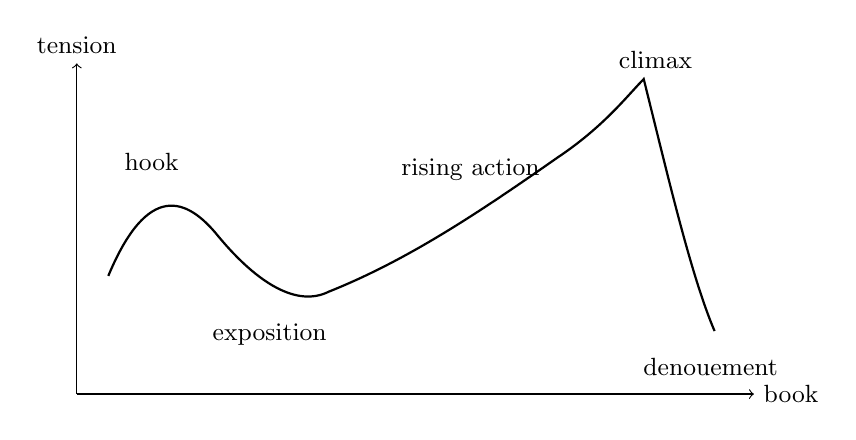
\begin{tikzpicture}[x=1cm,y=1cm]
\draw[->] (0,0) -- (8.6,0) node[right] {\small book};
\draw[->] (0,0) -- (0,4.2) node[above] {\small tension};
\draw[thick] (0.4,1.5)
  .. controls (0.9,2.7) and (1.4,2.5) .. (1.8,2.0)
  .. controls (2.3,1.4) and (2.8,1.1) .. (3.2,1.3)
  .. controls (4.2,1.7) and (5.1,2.3) .. (6.1,3.0)
  .. controls (6.7,3.4) and (7.0,3.8) .. (7.2,4.0)
  .. controls (7.5,2.8) and (7.8,1.5) .. (8.1,0.8);
\node at (0.95,2.95) {\small hook};
\node at (2.45,0.75) {\small exposition};
\node at (5.0,2.85) {\small rising action};
\node at (7.35,4.25) {\small climax};
\node at (8.05,0.35) {\small denouement};
\end{tikzpicture}
\caption{Powers の long-form tension graph を、transcript に基づいて schematic に再構成したもの。}
\end{figure}

denouement に関する Powers の gloss にも、notice すべきである。それは merely revelation ではない。book の course を通して tightened されてきた knot の loosening、あるいは blowing apart なのである。climax のあとには、reader が、その decisive choices が world の中で何を mean するのかを understand するために十分な aftermath を必要とする。

\subsection{Question \& Answer}

\paragraph{Question.} drama は、whole book の長さにわたって、どう structure を generate するのか。

\paragraph{Answer.} scene を animate する same collisions が、book の tension profile を determine するからである。form は drama の outside から impose されるのではない。rising and falling stakes の large-scale management なのである。

lecture はそこで終わらない。form から craft in use へと戻る。dialogue は、Powers によれば、empirically exact な speech ではない。bus の conversation を word for word transcribe し、それを fiction として print したなら、ほとんど unreadable であろう。good dialogue は stylized されている。その realism は stenographic ではなく conventional である。それが alive に sound するのは、ある given historical moment において speech についての reader の expectations を satisfy しつつ bend することを know しているからだ。

だからこそ Powers は、dialogue は heard aloud されるべきだと insist する。readers は subvocalize する。writers も line を ear で test すべきなのだ。これは only one valid style を produce するわけではない。Powers は Ann Patchett と Don DeLillo ほど different な writers を admire している。一方は speaking character の naturalness の中へ vanish することができるし、もう一方は人々が互いに talking past one another であることの absurdity を heighten できる。ear が holding しているなら、どちらも true でありうる。

lecture の終盤で、another practical principle が現れる。attention である。\emph{The Overstory} を書く前は、彼の house から office への path は、彼にとって simply ``tree, tree, tree'' だった、と Powers は言う。book の during には、それは species になった。red oak、maple、hornbeam。さらに deeper には、それは this individual tree になった。nearby の他のどの tree とも違う仕方で、何かを doing しているこの木へと。attention は granularity を increase し、granularity は prose を feed する。harder に look することは craft に peripheral なのではない。craft の sources の一つなのである。

lecture の recurring harness image は、ここで another form で return する。book は、head と heart、system と feeling、structure と emotion のあいだで forced な choice をさせられるべきではない。これらの elements が mutually に support し合い、lower down で made された decisions から emerge するとき、work は stronger になるのだ。

これによって Powers は solitude と daily practice へ至る。solitude は matter する。だが、それは one half of a rhythm としてのみである。world を quiet にし、scenes と sentences が traction を得られるようにするために、人は solitude に enter する。ついで solitude を leave し、その products を world に against してもう一度 test する。useful な late summary は、
\begin{equation}
\text{solitude} \to \text{composition} \to \text{return to the world} \to \text{correction}.
\end{equation}
となる。career の early には discipline は numerical だった。
\begin{equation}
1000\ \text{words/day}.
\end{equation}
later には、accountability は change する。task は、merely self から quota を extract することではなく、living world の中に be することになり、weather と calendar を check し、その日の amazement と instruction がどこにあるのかを ask することになる。そのとき sentences は、purely forced な output としてではなく、attention の supporting consequence として come するのである。

したがって lecture は、rigid な method ではなく、larger cycle をもって終わる。writing は、pressure と replenishment のあいだ、form と perception のあいだ、inward making と outward correction のあいだを move する。その final rhythm は、sentences についての any local tip と同じくらい重要なのである。

\section{まとめ}

Powers は、bag of advice ではなく chain を与えてくれる。character は pressure のもとで visible になる。pressure は drama を yield する。drama は inward なものから interpersonal なものへ、そこから environmental または metaphysical なものへと widen する。fiction が matter するのは、information alone では values は shift しないからである。story は affect と identification を recruit する。voice は words、register、syntax、predication から arise する。description は attention、expectation、controlled surprise によって work する。writer、reader、world が continue to move する以上、revision は決して本当に end しない。whole book の scale では、drama は tension の management を通じて form になる。そして writing life の scale では、work は solitude と living world とのあいだの repeated exchange によって proceed する。